\documentclass[conference]{IEEEtran}
\IEEEoverridecommandlockouts
% The preceding line is only needed to identify funding in the first footnote. If that is unneeded, please comment it out.
\usepackage{cite}
\usepackage{amsmath,amssymb,amsfonts}
\usepackage{algorithmic}
\usepackage{graphicx}
\usepackage{textcomp}
\usepackage{xcolor}
\usepackage{orcidlink}
\usepackage{booktabs}
\usepackage{multirow}
\def\BibTeX{{\rm B\kern-.05em{\sc i\kern-.025em b}\kern-.08em
    T\kern-.1667em\lower.7ex\hbox{E}\kern-.125emX}}
\begin{document}

\title{OCQR: Class-Conditional Conformalized Quantile Regression for Ordinal Classification}

% \author{Anonymous}
\author{\IEEEauthorblockN{Jinsu Hong\orcidlink{0009-0002-4383-1376}}
\IEEEauthorblockA{\textit{Department of Computer Science} \\
\textit{Georgia State University}\\
Atlanta, USA \\
jhong36@gsu.edu
}
\and
\IEEEauthorblockN{Chetraj Pandey\orcidlink{0000-0002-4699-4050}}
\IEEEauthorblockA{\textit{Department of Computer Science} \\
\textit{Texas Christian University} \\
Fort Worth, TX, USA \\
c.pandey@tcu.edu}
\and
\IEEEauthorblockN{Berkay Aydin\orcidlink{0000-0002-9799-9265}}
\IEEEauthorblockA{\textit{Department of Computer Science} \\
\textit{Georgia State University}\\
Atlanta, USA \\
baydin2@gsu.edu}
}

\maketitle

\begin{abstract}
High-stakes scientific and real-world applications require reliable uncertainty quantification beyond deterministic point predictions. Conformal prediction (CP) provides finite-sample coverage guarantees under exchangeability, but standard classification-based CP methods generally treat class labels as nominal and often produce disjoint prediction sets that ignore ordinal structure. Existing ordinal CP methods have primarily focused on order-aware or contiguous prediction-set construction, while class-conditional coverage for individual ordinal classes has received comparatively less attention. This limitation is particularly relevant for imbalanced ordinal data, where rare classes may exhibit substantially lower empirical coverage than frequent classes. We propose Ordinal Conformalized Quantile Regression (OCQR), a model-agnostic framework that combines conformalized quantile regression with true-label Mondrian calibration. OCQR computes class-specific conformal corrections and evaluates ordinal candidates in a numeric target space. Under within-class exchangeability and target-label consistency, OCQR provides finite-sample class-conditional coverage for each ordinal class. An add-only ordinal hull and conservative fallback produce nonempty, contiguous prediction sets while preserving the coverage guarantee and requiring no ordinal-specific modification to the backbone architecture. We evaluate OCQR on UTKFace, RetinaMNIST, and a highly imbalanced solar flare forecasting dataset. We compare OCQR with existing methods and examine the effects of class-specific calibration and ordinal post-processing through ablation studies. Experimental results show that OCQR provides a favorable coverage-set size tradeoff across three datasets. It improves worst-class coverage over the compact nominal baselines by 18.4-63.0 percentage points, while yielding smaller prediction sets than the conservative high-coverage baselines.
\end{abstract}

\begin{IEEEkeywords}
Conformal prediction, uncertainty quantification, ordinal classification,
class-conditional coverage, quantile regression
\end{IEEEkeywords}

\section{Introduction}
Reliable uncertainty quantification is important for machine learning systems deployed in high-stakes applications, where deterministic point predictions may provide insufficient information for decision-making. Set-valued predictions can provide additional information by representing multiple plausible outcomes rather than a single predicted class. In ordinal classification, however, the predicted outcomes also follow a natural order, and set-valued predictions should account for this ordered structure. Representative applications include disease severity grading, age estimation, risk assessment, and space weather forecasting.

As predictive models are increasingly trained on large-scale, high-dimensional, and multimodal datasets, obtaining reliable uncertainty estimates without substantially increasing training cost becomes important. Conformal prediction (CP) provides a distribution-free framework for constructing prediction sets with finite-sample coverage guarantees under exchangeability \cite{vovk1999cp}. Its model-agnostic formulation and relatively low calibration cost make it suitable for uncertainty quantification in modern machine learning systems. In particular, split conformal prediction can be applied to a pre-fitted predictive model without repeated model retraining, resulting in relatively low additional computational cost \cite{zhou2025conformal}. This property is attractive for large-scale learning problems involving high-dimensional or multimodal data, where training the underlying model can be computationally expensive and repeatedly fitting multiple models for uncertainty quantification may be impractical \cite{grasselli2025uncertainty}. However, standard classification-based CP methods do not explicitly account for class ordering and may produce disjoint prediction sets that include nonadjacent classes while excluding intermediate ones. For example, a prediction set may contain low- and high-severity classes but omit the classes between them \cite{lu2022oaps,zhang2026cps}. Such prediction sets are inconsistent with the ordered label space and can be difficult to interpret in practical applications. 

Recent studies have proposed ordinal CP methods that construct order-aware or contiguous prediction sets. Existing methods include conformal predictions for ordinal classification (COPOC) \cite{dey2023copoc} and ordinal adaptive prediction sets (OAPS) \cite{lu2022oaps}. These methods extend conformal uncertainty quantification to ordinal classification. OAPS constructs contiguous prediction sets from classifier outputs through an order-aware post-hoc procedure, but its coverage guarantee is marginal rather than class-conditional \cite{lu2022oaps}. COPOC is designed around a specialized ordinal prediction model and training procedure, which may limit its direct application to pretrained classifiers. Existing ordinal CP methods primarily address the structural consistency of ordinal prediction sets. Our work addresses a complementary objective by targeting class-conditional coverage while preserving ordinal contiguity. This distinction is important under severe class imbalance, where marginal coverage may conceal under-coverage of rare classes.

To address these limitations, we propose Ordinal Conformalized Quantile Regression (OCQR), a model-agnostic framework for ordinal classification. OCQR represents ordinal outcomes in a numeric target space and combines conformalized quantile regression (CQR) \cite{romano2019cqr} with true-label Mondrian calibration \cite{vovk2012conditional,vovk2005algorithmic}. The method computes class-specific conformal corrections and evaluates each ordinal candidate using its class-specific correction. Under the assumptions specified in Section~\ref{methodology}, OCQR provides finite-sample class-conditional coverage. We evaluate OCQR on three ordinal prediction tasks: UTKFace \cite{utkface-zhifei2017cvpr} for facial age estimation, RetinaMNIST \cite{medmnistv2} for diabetic-retinopathy severity grading, and a highly imbalanced solar flare forecasting dataset \cite{roy2026suryabench}. Across all datasets, we compare OCQR with standard and ordinal conformal prediction baselines in terms of marginal coverage, class-conditional coverage, prediction-set size, and contiguity.

The main contributions of this paper are as follows:
\begin{itemize}
\item We propose OCQR, a model-agnostic ordinal conformal framework that combines quantile regression with true-label Mondrian calibration.

\item We develop a candidate-wise inference procedure that evaluates each ordinal class using its corresponding class-specific conformal correction and provides finite-sample class-conditional coverage under within-class exchangeability and target-label consistency.

\item We construct nonempty and contiguous ordinal prediction sets using candidate-specific bin intersection, a conservative empty-set fallback, and an add-only ordinal hull that preserves the coverage guarantee.

\item We evaluate OCQR on multiple ordinal classification benchmarks, comparing it with standard and ordinal conformal prediction methods in terms of marginal and class-conditional coverage, prediction-set efficiency, and contiguity.

\end{itemize}

The remainder of this paper is organized as follows. Section~\ref{relatedwork} reviews related work on classification, class-conditional, and ordinal conformal prediction. Section~\ref{methodology} presents OCQR and its class-conditional coverage guarantee. Section~\ref{sec:experimental_setup} describes the experimental setup, and Section~\ref{results} presents the results and discussion. Section~\ref{conclusion} concludes the paper.

\section{Related Work}
\label{relatedwork}
This section reviews prior work most relevant to OCQR from four perspectives: conformal prediction for multiclass classification, conformalized quantile regression, class-conditional conformal prediction, and conformal prediction for ordinal classification. These directions respectively provide the classification, numeric-target, conditional-coverage, and ordinal-structure foundations on which OCQR builds.

\subsection{Conformal Prediction for Classification}
\label{subsec:cp_classification}

Several conformal prediction methods have been developed for multiclass classification. The Least Ambiguous set-valued Classifier (LAC) uses the nonconformity score \(1-\widehat{p}_y(x)\), where \(\widehat{p}_y(x)\) is the predicted probability assigned to the true class \cite{sadinle2019least}. After calibration, classes with sufficiently high predicted probabilities are included in the prediction set. Adaptive Prediction Sets (APS) rank classes by their predicted probabilities and construct a prediction set by accumulating probability mass until a calibrated threshold is reached \cite{angelopoulos2020uncertainty,romano2020classification}. Both methods provide marginal coverage under the standard split-conformal assumptions, but they treat the label space as nominal. They do not distinguish between adjacent and distant ordinal classes and may produce fragmented prediction sets that contain nonadjacent labels while excluding intermediate classes.

\subsection{Conformalized Quantile Regression}
\label{subsec:cqr}
Conformalized Quantile Regression (CQR) combines quantile regression with split-conformal calibration to construct prediction intervals for continuous targets \cite{romano2019cqr}. Because CQR operates in a numeric target space, it provides a numeric representation that can be used for ordered outcomes. However, standard CQR produces continuous intervals rather than discrete ordinal prediction sets and does not directly provide class-conditional coverage for ordinal labels. OCQR builds on this numeric formulation to construct class-conditional prediction sets for ordinal outcomes.

\subsection{Class-Conditional Conformal Prediction}
\label{subsec:mondrian_cp}
Marginal coverage controls the probability that a prediction set contains the true label when averaged over the full data distribution, but it does not guarantee that the target coverage level is attained separately for each class. In an imbalanced classification problem, high coverage for frequent classes can compensate for undercoverage in rare classes while the overall marginal target remains satisfied. 

Mondrian conformal prediction addresses group-specific coverage by partitioning calibration observations according to a predefined taxonomy and estimating a separate conformal correction within each group \cite{vovk2005algorithmic,vovk2012conditional}. When the taxonomy is defined using the true class label, calibration scores are grouped by class. Under within-class exchangeability, class-specific split-conformal calibration provides finite-sample class-conditional coverage.

However, standard Mondrian conformal prediction does not account for the ordering of the class labels and may produce disjoint prediction sets. Class-specific coverage and ordinal contiguity need to be addressed jointly.

\subsection{Conformal Prediction for Ordinal Classification}
\label{subsec:ordinal_cp}

Recent studies have proposed conformal methods that explicitly incorporate the ordering of class labels. Ordinal Adaptive Prediction Sets (OAPS) modify probability-based conformal set construction by expanding the prediction set through neighboring ordinal classes while preserving label contiguity \cite{lu2022oaps}. While this approach constructs contiguous prediction sets, its coverage guarantee is marginal rather than class-conditional. As a result, the empirical coverage can differ across classes, with rare classes potentially undercovered even when dominant classes are well covered.

Conformal Predictions for Ordinal Classification (COPOC) constructs ordinal conformal prediction sets using a unimodal probability construction over the ordered classes \cite{dey2023copoc}. This structure facilitates the construction of contiguous prediction sets but requires an ordinal-specific prediction model and associated training procedure. As a result, its direct application to a pretrained classifier may require modifying the output layer or retraining the classifier. 

Prior ordinal CP methods such as OAPS and COPOC focus on order-aware or contiguous prediction-set construction under marginal coverage guarantees. Our work builds on this objective by targeting class-conditional coverage for individual ordinal classes while preserving prediction-set contiguity. 

\begin{figure*}
    \centering
    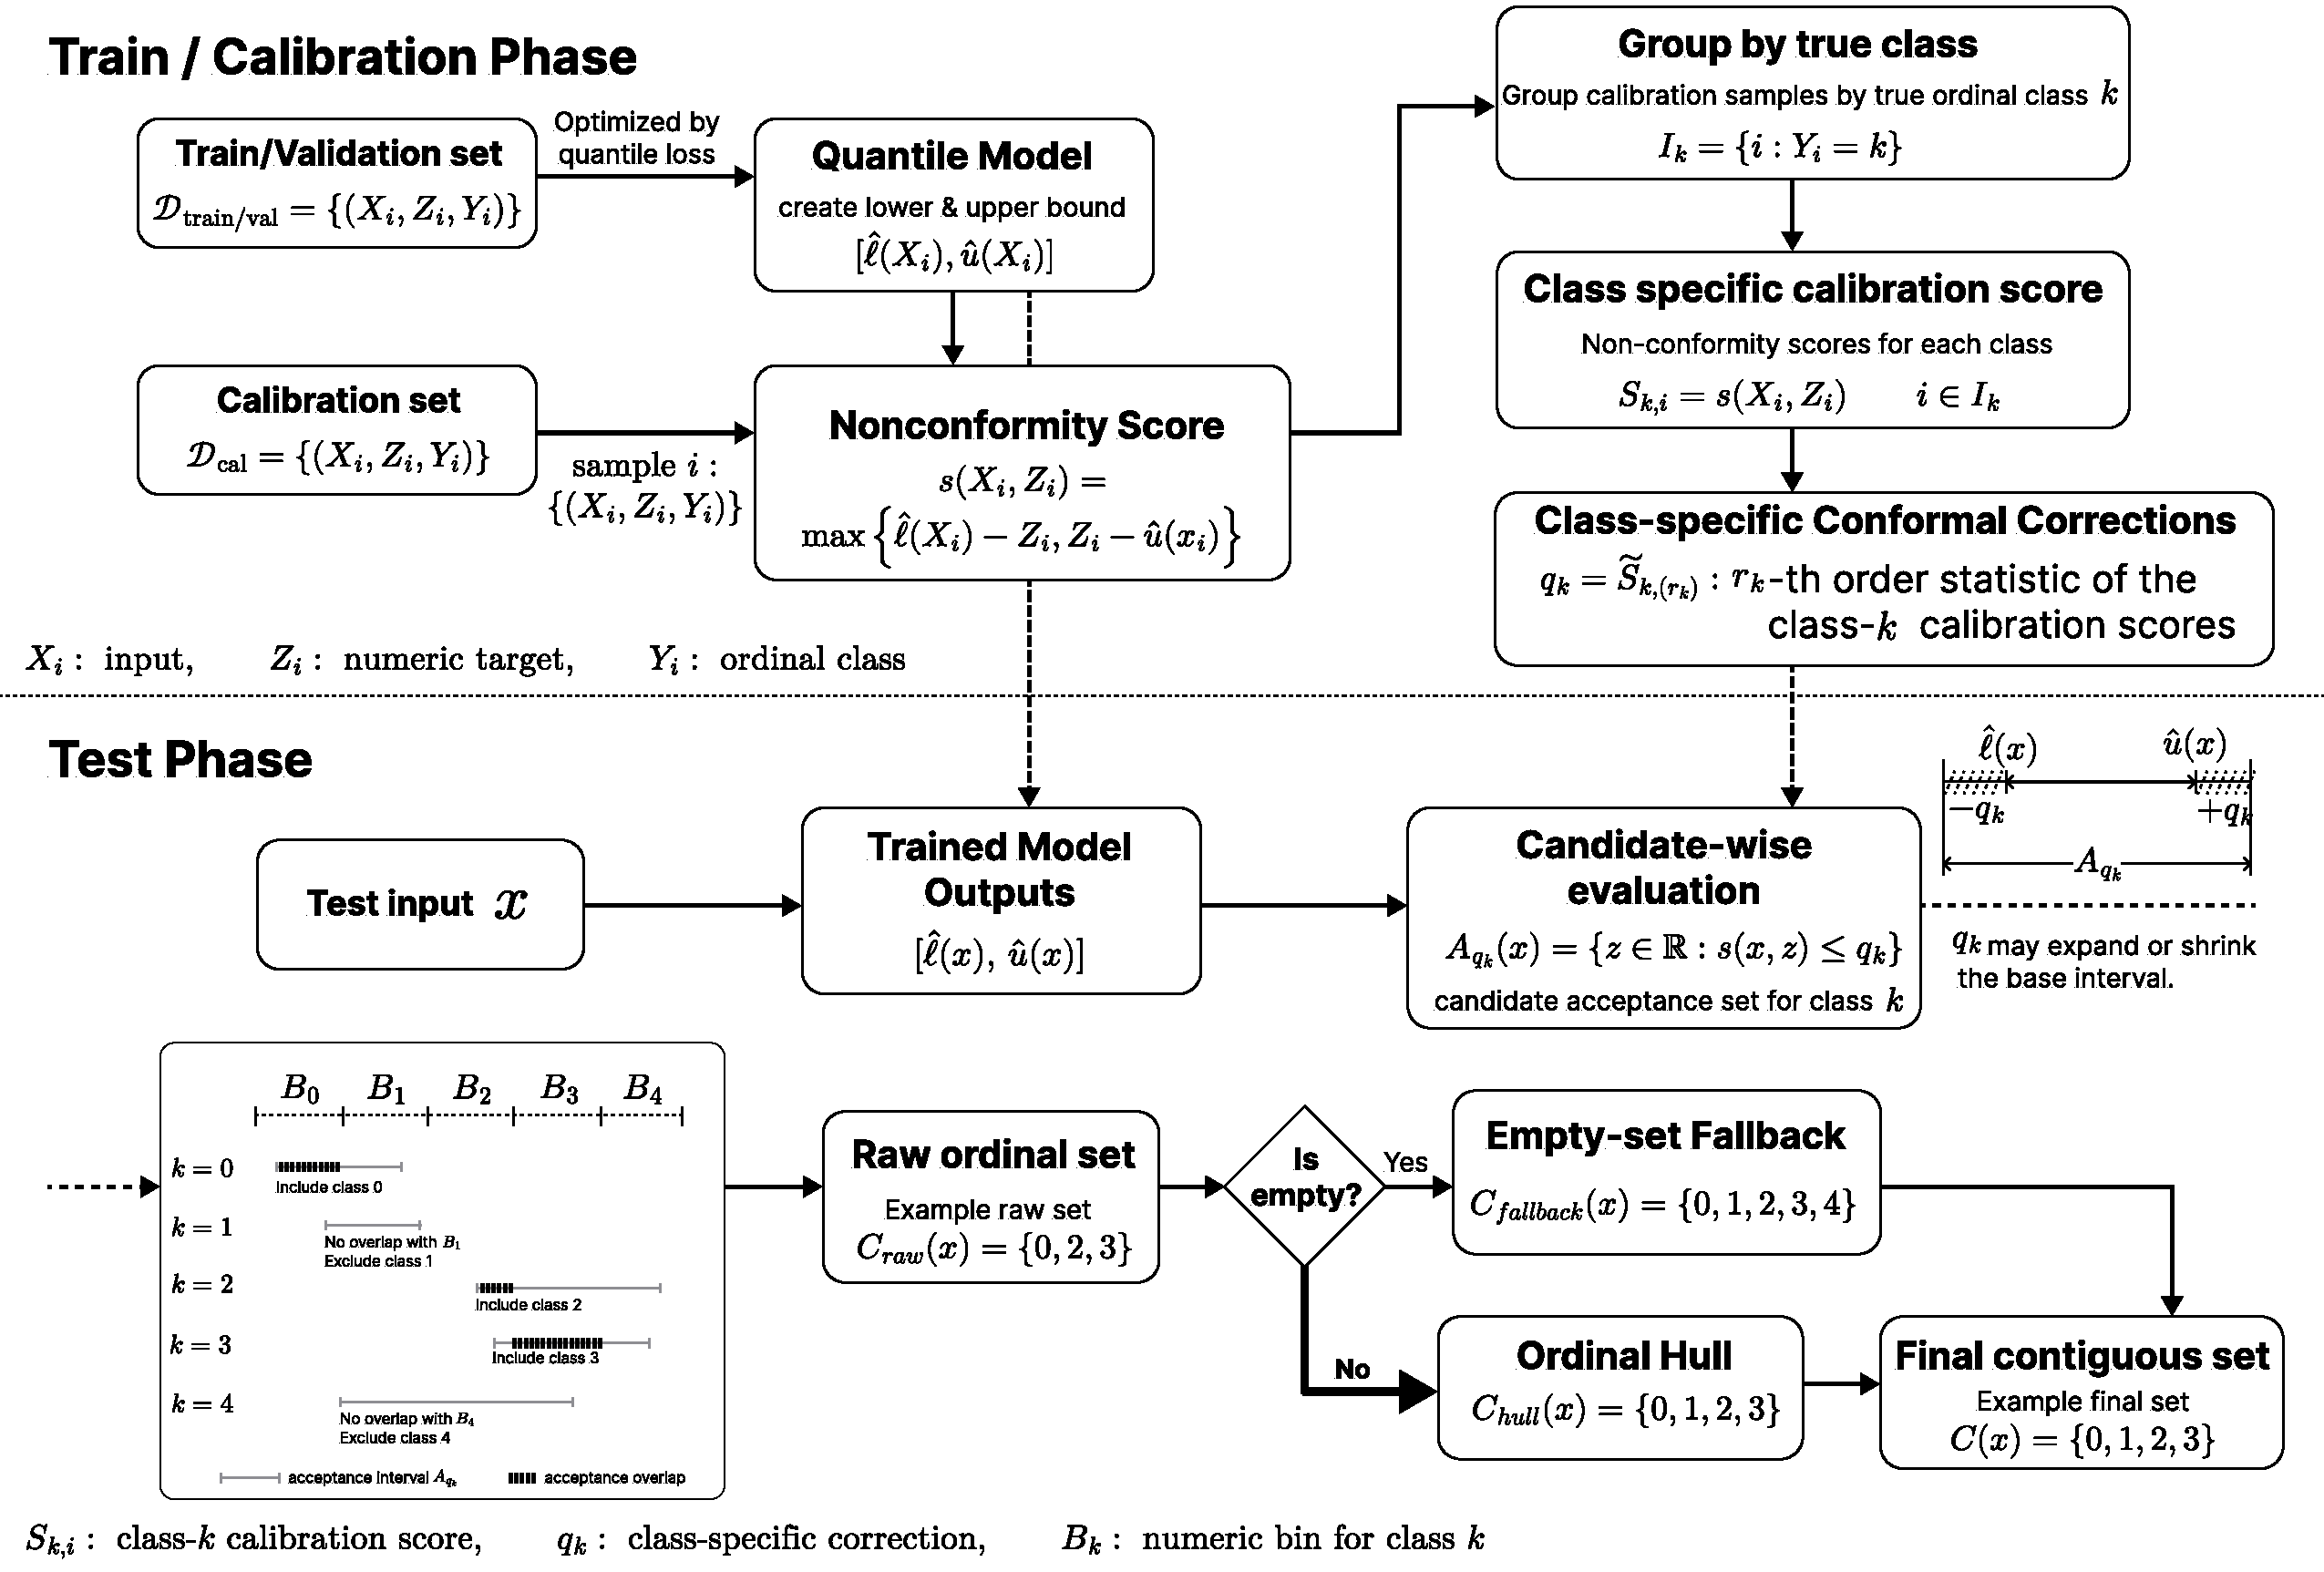
\includegraphics[width=0.98\linewidth]{OCQR.pdf}
    \caption{Overview of the OCQR framework. During training and calibration, the quantile model is fitted and class-specific conformal corrections are estimated using true-label Mondrian calibration. At inference, each ordinal class is evaluated with its own correction, and the raw prediction set is converted into a nonempty contiguous set using the fallback and ordinal hull.}
    \label{fig:ocqr-concept}
\end{figure*}

\section{Proposed Methodology}
\label{methodology}

This section presents Ordinal Conformalized Quantile Regression (OCQR). OCQR combines quantile-based modeling in a numeric target space with true-label Mondrian calibration. It evaluates each ordinal class using a class-specific conformal correction and maps the resulting numeric acceptance sets to a nonempty contiguous ordinal prediction set.

\subsection{Problem Formulation}
\label{subsec:problem_formulation}

Let an observation be represented by \((X,Z,Y)\), where \(X\in\mathcal{X}\) is the model input, \(Z\in\mathbb{R}\) is the numeric target used for quantile regression and conformal calibration, and \(Y\in\mathcal{Y}=\{0,\ldots,K-1\}\) is the ordinal class label. For any \(k\in\mathcal{Y}\), let \(k\) denote an ordinal class index. Fixed thresholds  \(b_1<\cdots<b_{K-1}\) define the ordinal bins \(B_0,\ldots,B_{K-1}\), with the first and last bins extending to \(-\infty\) and \(+\infty\), respectively. The thresholds and target representation are fixed before conformal calibration. We require target-label consistency between the ordinal label \(Y\) and the numeric target \(Z\): if \(Y=k\), then \(Z\) must lie in the predefined numeric bin \(B_k\) associated with class \(k\),
\begin{equation}
Y=k \Longrightarrow Z\in B_k.
\label{eq:target_label_consistency}
\end{equation}
The same label \(Y\) is used to form the true-label Mondrian calibration groups. The numeric target \(Z\) is used to train the quantile regression model and compute the conformal score, whereas the supplied ordinal label \(Y\) defines the ordinal prediction task and the true-label Mondrian calibration groups. 

% We consider two target settings. (i) When an ordinal label is accompanied by a related numeric measurement, \(Z\) is the measured quantity or an order-preserving transformation of it, and the ordinal bins \(B_k\) are chosen so that Eq.~\eqref{eq:target_label_consistency} holds. (ii) For datasets that provide only ordinal labels but no separate numeric target, we construct \(Z\) using an ordinal embedding \(Z=e(Y)\). In this work, we use the class-index embedding \(e(k)=k\), which preserves the class ordering. This embedding is a modeling choice rather than a requirement for the class-conditional coverage guarantee. 
\subsection{Quantile Regression and Nonconformity Score} \label{subsec:quantile_model}
In conformal prediction, miscoverage refers to the event that the prediction set fails to contain the true label. Let \(\alpha\in(0,1)\) denote the target miscoverage level. OCQR estimates lower and upper conditional quantiles of \(Z\), denoted by \(\widehat q_{\tau_L}(x)\) and \(\widehat q_{\tau_U}(x)\), where input \(x\in\mathcal{X}\),  \(\tau_L=\alpha/2\), and \(\tau_U=1-\alpha/2\).  For quantile level \(\tau\), let \(r=z-\widehat q_{\tau}(x)\). The quantile loss is
\begin{equation}
\rho_{\tau}(r)
=
\max\{\tau r, (\tau-1)r\}.
\label{eq:quantile_loss}
\end{equation}
To correct quantile crossing, where the predicted lower quantile  \(\widehat q_{\tau_L}(x)\) exceeds the upper quantile \(\widehat q_{\tau_U}(x)\), we order the two predicted endpoints as 
\begin{equation}
\begin{aligned}
\widehat\ell(x)
&=
\min\{\widehat q_{\tau_L}(x),\widehat q_{\tau_U}(x)\},\\
\widehat u(x)
&=
\max\{\widehat q_{\tau_L}(x),\widehat q_{\tau_U}(x)\}.
\end{aligned}
\label{eq:ordered_endpoints}
\end{equation}
All subsequent calibration and prediction steps use these ordered endpoints. OCQR uses the CQR nonconformity score
\begin{equation}
s(x,z) =
\max\left\{\widehat\ell(x)-z, z-\widehat u(x)\right\}.
\label{eq:cqr_score}
\end{equation}
At inference time, for a test input \(x\) and conformal correction \(q\), define the numeric acceptance set $A_q(x)$ as:
\begin{equation}
A_q(x) =
\left\{
z\in\mathbb{R}: s(x,z)\le q
\right\}.
\label{eq:acceptance_set}
\end{equation}
For finite \(q\), this set is
\begin{equation}
A_q(x)=
\begin{cases}
[\widehat\ell(x)-q,\widehat u(x)+q], &
  \widehat\ell(x)-q\le\widehat u(x)+q, \\[3pt]
  \varnothing, &
\text{otherwise}.
\end{cases}
\label{eq:score_inversion}
\end{equation}
For \(q=+\infty\), we define \(A_q(x)=\mathbb{R}\). The fitted model and all data-dependent method choices are fixed using only training and validation data. Calibration data are used only to compute the conformal corrections, and test data are reserved for final evaluation.

\subsection{True-Label Mondrian Calibration}
\label{subsec:mondrian_calibration}
Let the calibration set be \(\mathcal{D}_{\mathrm{cal}}=\{(X_i,Z_i,Y_i)\}_{i=1}^{n}\). For each class \(k\), let \(\mathcal{I}_k=\{i:Y_i=k\}\) denote the indices of calibration examples with true class \(k\), and let \(N_k=\lvert\mathcal{I}_k\rvert\) be the number of calibration examples in that class. The groups are formed using the supplied true ordinal labels rather than predicted labels. For \(i\in\mathcal{I}_k\), the calibration score is \(S_{k,i}=s(X_i,Z_i)\). We define the class-specific conformal rank as:
\begin{equation}
r_k
=
\left\lceil
(N_k+1)(1-\alpha)
\right\rceil.
\label{eq:conformal_rank}
\end{equation}
The class-specific nonconformity score multiset is augmented with one \(+\infty\) value, \(\widetilde{\mathcal{S}}_k=\{S_{k,i}:i\in\mathcal{I}_k\}\cup\{+\infty\}\). Let \(\widetilde S_{k,(j)}\) denote its \(j\)-th order statistic. The class-specific conformal correction is
\begin{equation}
q_k=
\widetilde S_{k,(r_k)}.
\label{eq:class_correction}
\end{equation}
We use the exact discrete order statistic consistent with the finite-sample split-conformal rank construction; no interpolation is applied, and tied scores are retained without tie-breaking. Under the augmented construction, \(q_k=+\infty\) when the requested rank is not supported by a finite class-specific score. When \(q_k=+\infty\), the acceptance set for class \(k\) becomes \(\mathbb{R}\), so class \(k\) is included for every test input. This guarantees inclusion of class \(k\) but may increase prediction-set size.

\subsection{Candidate-Specific Ordinal Prediction}
\label{subsec:candidate_prediction}
At test time, the true class is unknown. OCQR therefore evaluates every candidate class \(k\) using its corresponding correction \(q_k\). For a test input \(x\in\mathcal{X}\), the raw ordinal prediction set is
\begin{equation}
C_{\mathrm{raw}}(x)
=
\left\{
k\in\mathcal{Y}:
A_{q_k}(x)\cap B_k\neq\varnothing
\right\}.
\label{eq:raw_set}
\end{equation}
For a finite nonempty interval \(A_{q_k}(x)=[L_k(x),U_k(x)]\), candidate \(k\) is included when \(U_k(x)\ge b_k\) and \(L_k(x)<b_{k+1}\). This procedure may produce a fragmented raw set, such as \(\{k_1,k_3,k_4\}\), in which an intermediate class \(k_2\) is omitted.

\subsection{Nonempty Fallback and Ordinal Hull}
\label{subsec:ordinal_hull}
If the raw candidate set is empty, OCQR applies the conservative fallback
\begin{equation}
\widetilde C_{\mathrm{raw}}(x)
=
\begin{cases}
C_{\mathrm{raw}}(x),
&
C_{\mathrm{raw}}(x)\neq\varnothing, \\[3pt]
\mathcal{Y},
&
C_{\mathrm{raw}}(x)=\varnothing.
\end{cases}
\label{eq:empty_fallback}
\end{equation}
The final prediction set is 
\begin{equation}
C(x)
=
\left\{
j\in\mathcal{Y}:
\min\widetilde C_{\mathrm{raw}}(x)\le j\le\max \widetilde C_{\mathrm{raw}}(x)
\right\}.
\label{eq:final_prediction_set}
\end{equation}
Both operations only add labels, so \(C_{\mathrm{raw}}(x)\subseteq\widetilde C_{\mathrm{raw}}(x)\subseteq C(x)\). Therefore, the resulting prediction set is nonempty and contiguous.

\begin{table*}[t]
\centering
% \small
\caption{Dataset summary. Counts are the examples used by each experimental pipeline: frozen-manifest rows for UTKFace and RetinaMNIST, and image-available rows for solar flare after the documented target-label filtering.}
\label{tab:dataset_summary}
% \resizebox{\textwidth}{!}{%
\begin{tabular}{lllp{4.0cm}rrrr}
\toprule
Dataset & Input & Classes & Numeric target $Z$ & Train & Val. & Cal. & Test \\
\midrule
UTKFace & $128\times128\times3$& 5 & Chronological age (years) & 14{,}224 & 2{,}371 & 4{,}742 & 2{,}371 \\
RetinaMNIST & $28\times28\times 3$& 5 & Fixed class-index embedding& 756 & 120 & 324 & 400 \\
Solar flare & $224\times224\times13$ & 5 & \(log_{10}(\texttt{max\_intensity})+9\)& 42{,}292 & 2{,}255 & 3{,}605 & 27{,}620 \\
\bottomrule
\end{tabular}
% }
\end{table*}

\subsection{Class-Conditional Coverage}
\label{subsec:coverage_guarantee}

Let \(\mathcal{F}\) denote the all information used to fit and select the prediction procedure before conformal calibration, including the training and validation data, fitted model, target representation and bin boundaries, selected hyperparameters, Mondrian taxonomy, and post-processing rules. These components are fixed without using the calibration or test observations.

\noindent\textbf{Theorem 1.}
Assume target-label consistency and, for each \(k\in\mathcal{Y}\), within-class exchangeability of the class-\(k\) calibration scores and the corresponding test score conditional on \(\mathcal{F}\). Under the OCQR construction defined above, for every \(k\in\mathcal{Y}\),
\begin{equation}
\Pr\left\{
Y_{n+1}\in C(X_{n+1})
\mid
\mathcal{F},Y_{n+1}=k
\right\}
\ge 1-\alpha.
\label{eq:conditional_coverage}
\end{equation}
Consequently,
\begin{equation}
\Pr\left\{
Y_{n+1}\in C(X_{n+1})
\mid
Y_{n+1}=k
\right\}
\ge 1-\alpha.
\label{eq:label_conditional_coverage}
\end{equation}
The final prediction set is nonempty and contiguous.

\noindent\textit{Proof sketch.}
Conditional on \(\mathcal{F}\), \(N_k\), and \(Y_{n+1}=k\), the augmented split-conformal rank argument gives \(s(X_{n+1},Z_{n+1})\le q_k\) with probability at least \(1-\alpha\). On this event, the definition of \(A_{q_k}\) implies \(Z_{n+1}\in A_{q_k}(X_{n+1})\). Target-label consistency also gives \(Z_{n+1}\in B_k\), implying \(A_{q_k}(X_{n+1})\cap B_k\neq\varnothing\) and hence \(k\in C_{\mathrm{raw}}(X_{n+1})\). The fallback and ordinal hull only add labels and therefore preserve this inclusion. Averaging over \(N_k\) gives Eq.~\eqref{eq:conditional_coverage}, and averaging over \(\mathcal{F}\) gives Eq.~\eqref{eq:label_conditional_coverage}.

\section{Experimental Setup}
\label{sec:experimental_setup}
We evaluate OCQR on three ordinal classification tasks spanning facial age estimation, medical severity grading, and solar flare forecasting. This section describes the datasets and data splits, comparison baselines and ablation variants, model-training and calibration settings, and evaluation metrics used throughout the experiments. All methods are evaluated under a common experimental settings, with model selection completed before conformal calibration.


\subsection{Datasets}
\label{subsec:datasets}
We evaluate OCQR on three five-class ordinal classification tasks: facial age estimation on UTKFace \cite{utkface-zhifei2017cvpr}, diabetic-retinopathy severity grading on RetinaMNIST \cite{medmnistv2}, and solar flare forecasting on SuryaBench \cite{roy2026suryabench}. UTKFace uses an observed numeric target, RetinaMNIST uses a fixed class-index embedding, and solar flare uses an observed numeric target under a chronological data split. All datasets use fixed training, validation, calibration, and test splits. The data partitions remain unchanged across the five experimental seeds 0-4, which capture training randomness rather than split variability. Table~\ref{tab:dataset_class_counts} reports the class counts in the calibration and test splits for all three datasets, which are relevant to the class-conditional coverage evaluation. Model selection is completed before conformal calibration, and the test split is used only for final evaluation. 

\paragraph{UTKFace}
UTKFace contains cropped and aligned facial images with chronological age annotations \cite{utkface-zhifei2017cvpr}. We use age in years as $Z$ and the fixed ordinal bins $(-\infty,20)$, $[20,40)$, $[40,60)$, $[60,80)$, and $[80,+\infty)$. After excluding files whose age could not be parsed from the filename, the dataset contains 23{,}708 images with ages ranging from 1 to 116 years. We resize images to $128\times128$, normalize using the ImageNet mean and standard deviation \cite{deng2009imagenet}, and apply random horizontal flipping only during training. We construct stratified splits with 60\%/10\%/20\%/10\% of the images assigned to the training, validation, calibration, and test sets, respectively, while approximately preserving the ordinal class proportions in each subset. The split is performed at the image level, meaning that individual images, rather than subjects, are assigned to the four subsets. Because subject identifiers are unavailable, we cannot guarantee that images of the same individual are assigned to only one split.

\paragraph{RetinaMNIST}
RetinaMNIST contains \(28\times28\)-pixel RGB retinal fundus images with five ordered diabetic-retinopathy severity labels \cite{medmnistv2}. Because it provides no measured continuous target, we use the fixed embedding $Z=Y\in\{0,\ldots,4\}$ and midpoint bin boundaries $0.5$, $1.5$, $2.5$, and $3.5$. The official validation and test partitions contain 120 and 400 images, respectively. We stratify the official 1{,}080 image training partition into 756 training and 324 calibration images. We normalize each channel using mean \(0.5\) and standard deviation \(0.5\), and use no resizing or data augmentation.

\paragraph{Solar flare forecasting}
Solar flare forecasting is a highly imbalanced ordinal forecasting task that uses a 13-channel Solar Dynamics Observatory (SDO) image stack as input to predict flare activity over subsequent 24 hours \cite{roy2026suryabench}. The numeric target is $Z=\log_{10}(\texttt{max\_intensity})+9$, where \texttt{max\_intensity} is the maximum GOES X-ray flux in the 24-hour forecast window. The ordinal classes are FQ/A, B, C, M, and X, with bin boundaries $2$, $3$, $4$, and $5$ in this transformed coordinate. 

For each year from 2010 to 2019, calibration uses observations from January 1-14 and February 1-14, validation uses January 15-31, and training uses February 15-December 31. The future-test set contains all retained observations from 2020-2024. Thus, the development subsets use nonoverlapping calendar intervals within each year, while the test set is temporally separated from the 2010-2019 development period. Because the test period occurs strictly after the development period, we report solar flare coverage as empirical temporal-extrapolation performance rather than as evidence that calibration and test observations satisfy the exchangeability assumption required by the finite-sample guarantee.

\begin{table}[h]
\label{tab:dataset_class_counts}
\caption{Class counts in the calibration and test splits for each dataset.}
\begin{tabular}{llrrrrr}
\toprule
Dataset & Split & Class 0 & Class 1 & Class 2 & Class 3 & Class 4 \\
\midrule
Retina & Cal. & 146 & 38 & 62 & 58 & 20 \\
Retina & Test & 174 & 46 & 92 & 68 & 20 \\
\midrule
UTKFace & Cal. & 919 & 2{,}376 & 909 & 403 & 135 \\
UTKFace & Test & 459 & 1{,}189 & 454 & 202 & 67 \\
\midrule
Flare & Cal. & 626 & 960 & 1{,}352 & 626 & 41  \\
Flare & Test & 4{,}952 & 4{,}403 & 9{,}897 & 7{,}420 & 948  \\
\bottomrule
\end{tabular}
\end{table}

\subsection{Baselines and Ablations}
\label{subsec:baselines}

We compare OCQR with LAC \cite{sadinle2019least}, APS \cite{angelopoulos2020uncertainty,romano2020classification}, OAPS \cite{lu2022oaps}, and COPOC \cite{dey2023copoc}. LAC, APS, and OAPS use the same ResNet-18 Softmax backbone within each dataset; COPOC uses a separately trained ResNet-18 with its ordinal-specific nonparametric unimodal output construction. All methods use the same data split and common evaluation pipeline.

We evaluate five OCQR variants on all three datasets:
\begin{itemize}
    \item \textbf{OCQR-Pooled}: uses a single conformal correction estimated from the pooled calibration set instead of class-specific corrections.
    \item \textbf{OCQR-NoHull}: omits ordinal-hull closure and can therefore return noncontiguous prediction sets.
    \item \textbf{OCQR-NoFallback}: omits the empty-set fallback and can therefore return empty prediction sets.
    \item \textbf{OCQR-Raw}: omits both ordinal-hull closure and the empty-set fallback.
    \item \textbf{OCQR-Nonnegative}: replaces negative nonconformity scores with zero to assess sensitivity to the signed score definition.
\end{itemize}

Table~\ref{tab:ocqr_ablation_config} summarizes the corresponding configurations.

\begin{table}[h]
\centering
\small
\caption{OCQR ablation configurations.}
\label{tab:ocqr_ablation_config}
\begin{tabular}{lcccc}
\toprule
Variant & Class cal. & Hull & Fallback & Nonnegative \\
\midrule
Pooled      & \(\times\)    & \checkmark & \checkmark & \(\times\) \\
NoHull      & \checkmark    & \(\times\) & \checkmark & \(\times\) \\
NoFallback  & \checkmark    & \checkmark & \(\times\) & \(\times\) \\
Raw         & \checkmark    & \(\times\) & \(\times\) & \(\times\) \\
Nonnegative & \checkmark    & \checkmark & \checkmark & \checkmark \\
Standard    & \checkmark    & \checkmark & \checkmark & \(\times\) \\
\bottomrule
\end{tabular}
\end{table}

\begin{table*}[t]
\centering
% \small
\caption{Main benchmark comparison at $\alpha=0.1$. Values are mean $\pm$
standard deviation across five seeds. Solar flare forecasting results use a frozen
chronological future-test split and are empirical temporal-extrapolation
results, not evidence that calibration-test exchangeability holds.}
\label{tab:main_benchmark_results}
\begin{tabular}{llrrrrr}
\toprule
Dataset & Method & Marginal (\%) & Macro (\%) & Worst (\%) & Set size & Full set (\%) \\
\midrule
RetinaMNIST & LAC   & 89.7 $\pm$ 1.0 & 83.2 $\pm$ 1.8 & 63.0 $\pm$ 6.2 & 3.36 $\pm$ 0.10 & 29.5 $\pm$ 4.9 \\
RetinaMNIST & APS   & 99.8 $\pm$ 0.4 & 99.6 $\pm$ 0.5 & 98.7 $\pm$ 1.9 & 4.91 $\pm$ 0.15 & 93.2 $\pm$ 10.4 \\
RetinaMNIST & OAPS  & 90.0 $\pm$ 1.9 & 80.3 $\pm$ 2.7 & 37.0 $\pm$ 17.2 & 3.19 $\pm$ 0.10 & 15.8 $\pm$ 5.7 \\
RetinaMNIST & COPOC & 99.2 $\pm$ 0.5 & 98.5 $\pm$ 1.0 & 95.0 $\pm$ 3.5 & 4.74 $\pm$ 0.16 & 84.9 $\pm$ 9.2 \\
RetinaMNIST & OCQR  & 95.8 $\pm$ 1.2 & 93.3 $\pm$ 1.3 & 81.4 $\pm$ 4.7 & 4.04 $\pm$ 0.18 & 62.3 $\pm$ 9.5 \\
\midrule
UTKFace & LAC   & 90.9 $\pm$ 0.4 & 83.9 $\pm$ 1.6 & 66.4 $\pm$ 9.0 & 1.60 $\pm$ 0.04 & 0.0 $\pm$ 0.0 \\
UTKFace & APS   & 99.8 $\pm$ 0.2 & 99.6 $\pm$ 0.4 & 98.8 $\pm$ 1.0 & 3.41 $\pm$ 0.18 & 13.6 $\pm$ 7.2 \\
UTKFace & OAPS  & 91.1 $\pm$ 0.4 & 84.3 $\pm$ 2.2 & 68.7 $\pm$ 11.6 & 1.62 $\pm$ 0.05 & 0.1 $\pm$ 0.1 \\
UTKFace & COPOC & 99.8 $\pm$ 0.1 & 99.5 $\pm$ 0.4 & 98.2 $\pm$ 1.6 & 3.38 $\pm$ 0.07 & 18.4 $\pm$ 3.6 \\
UTKFace & OCQR  & 98.7 $\pm$ 0.2 & 98.1 $\pm$ 0.4 & 96.7 $\pm$ 0.8 & 2.35 $\pm$ 0.06 & 0.0 $\pm$ 0.1 \\
\midrule
Solar flare & LAC   & 87.1 $\pm$ 0.7 & 73.9 $\pm$ 2.7 & 10.0 $\pm$ 15.1 & 1.83 $\pm$ 0.05 & 0.0 $\pm$ 0.0 \\
Solar flare & APS   & 98.5 $\pm$ 0.1 & 95.7 $\pm$ 1.5 & 81.9 $\pm$ 9.0 & 2.96 $\pm$ 0.04 & 0.6 $\pm$ 0.5 \\
Solar flare & OAPS  & 86.6 $\pm$ 0.5 & 72.7 $\pm$ 1.7 & 5.8 $\pm$ 8.8 & 1.82 $\pm$ 0.04 & 0.0 $\pm$ 0.0 \\
Solar flare & COPOC & 97.0 $\pm$ 0.9 & 90.1 $\pm$ 4.8 & 55.6 $\pm$ 24.4 & 3.07 $\pm$ 0.18 & 0.3 $\pm$ 0.3 \\
Solar flare & OCQR  & 89.6 $\pm$ 5.4 & 88.4 $\pm$ 6.2 & 73.0 $\pm$ 17.8 & 2.60 $\pm$ 0.11 & 0.0 $\pm$ 0.0 \\
\bottomrule
\end{tabular}
\end{table*}


\subsection{Implementation Details}
\label{subsec:implementation_details}
All experiments use \(\alpha=0.1\) and five training seeds, \(0,\ldots,4\). Each seed initializes the Python, NumPy, and PyTorch CPU/CUDA random-number generators and the shuffled training-data loader. Thus, the seeds vary model initialization, minibatch order, and stochastic training augmentation, while the data split, bin thresholds, hyperparameters, calibration rule, and evaluation protocol remain fixed. The five seeds share the same fixed data split within each dataset. OCQR predicts the \(0.05\) and \(0.95\) conditional quantiles, which define its lower and upper endpoints.

For RetinaMNIST and UTKFace, we use ResNet-18 backbones with dropout \(0.5\), AdamW with learning rate \(10^{-4}\) and weight decay \(0.01\), batch size 64, and at most 100 training epochs. For solar flare forecasting, we use a 13-channel ResNet-18 with dropout \(0.5\), AdamW with learning rate \(5\times10^{-5}\) and weight decay \(0.01\), batch size 64, at most 300 epochs, and a cosine learning-rate schedule with a warm-up ratio of \(0.1\). All ResNet-18 models are trained from random initialization without pretrained weights. Early stopping with patience=\(3\) and checkpoint selection are based on minimum validation pinball loss for OCQR and validation cross-entropy for the classification models.

The implementation uses Python 3.11, PyTorch 2.6, CUDA 12.4, and PyTorch Lightning. Code, configurations, and fixed data splits are available at \url{https://github.com/JinsuHongg/ordinal-cqr}.

\subsection{Evaluation Metrics}
\label{subsec:evaluation_metrics}

All experiments target a nominal coverage \(1-\alpha=0.9\). We report marginal coverage, macro class-conditional coverage, worst-class coverage, mean prediction-set size, and full-set rate. The full-set rate is the proportion of test examples for which \(C(X)=\mathcal{Y}\). For class $k$, empirical class coverage is
\begin{equation}
\widehat{\mathrm{Cov}}_k
=
\frac{1}{n_k}
\sum_{i:Y_i=k}
\mathbf{1}\{Y_i\in C(X_i)\},
\label{eq:empirical_class_coverage}
\end{equation}
where \(n_k\) is the number of test examples in class \(k\). Macro coverage is the mean of \(\widehat{\mathrm{Cov}}_k\) over the five classes, and worst-class coverage is their minimum. All test sets contain every class. We report each metric as mean \(\pm\) standard deviation across five runs. For the ablation analysis, we report the rates of empty and fragmented prediction sets to assess the fallback and ordinal hull.

\section{Results and Discussion} \label{results}
\subsection{Overall Performance}
Table~\ref{tab:main_benchmark_results} summarizes the results over five runs with fixed data splits and different training seeds. The results show a coverage-efficiency tradeoff. APS and COPOC attain the highest marginal, macro, and worst-class coverage on RetinaMNIST and UTKFace, but they also produce the largest prediction sets. LAC and OAPS produce substantially smaller sets, yet their marginal coverage masks class-conditional undercoverage. OCQR lies between these two regimes: it improves macro and worst-class coverage relative to LAC and OAPS while producing smaller prediction sets than APS and COPOC.

On RetinaMNIST, OCQR achieves marginal coverage of \(95.8\%\pm1.2\%\), macro class coverage of \(93.3\%\pm1.3\%\), and worst-class coverage of \(81.4\%\pm4.7\%\). Its mean set size is \(4.04\pm0.18\). APS and COPOC attain higher worst-class coverage of \(98.7\%\pm1.9\%\) and \(95.0\%\pm3.5\%\), respectively, but their mean set sizes increase to \(4.91\pm0.15\) and \(4.74\pm0.16\) out of five classes. By contrast, LAC and OAPS have smaller mean set sizes of \(3.36\pm0.10\) and \(3.19\pm0.10\), but their worst-class coverage falls to \(63.0\%\pm6.2\%\) and \(37.0\%\pm17.2\%\).

The UTKFace results show a more favorable tradeoff for OCQR. OCQR obtains marginal coverage of \(98.7\%\pm0.2\%\), macro class coverage of \(98.1\%\pm0.4\%\), and worst-class coverage of \(96.7\%\pm0.8\%\), with a mean set size of \(2.35\pm0.06\). APS and COPOC again attain slightly higher coverage, but require mean set sizes of \(3.41\pm0.18\) and \(3.38\pm0.07\), respectively. LAC and OAPS return much smaller sets, approximately \(1.60\) classes on average, while their worst-class coverage is only \(66.4\%\pm9.0\%\) and \(68.7\%\pm11.6\%\). These results show that marginal coverage near the nominal level does not necessarily imply comparable coverage across ordinal classes.

The solar flare forecasting results exhibit a different pattern under the chronological future-test setting. OCQR achieves marginal coverage of \(89.6\%\pm5.4\%\), macro class coverage of \(88.4\%\pm6.2\%\), and worst-class coverage of \(73.0\%\pm17.8\%\), with a mean set size of \(2.60\pm0.11\). APS attains substantially higher coverage, with marginal, macro, and worst-class coverage of \(98.5\%\pm0.1\%\), \(95.7\%\pm1.5\%\), and \(81.9\%\pm9.0\%\), respectively, but requires a larger mean set size of \(2.96\pm0.04\). COPOC also produces a larger mean set size of \(3.07\pm0.18\), while its worst-class coverage decreases to \(55.6\%\pm24.4\%\). LAC and OAPS return smaller sets, with mean sizes of \(1.83\pm0.05\) and \(1.82\pm0.04\), but their worst-class coverage drops sharply to \(10.0\%\pm15.1\%\) and \(5.8\%\pm8.8\%\), respectively. OCQR achieves higher mean worst-class coverage than LAC, OAPS, and COPOC while maintaining smaller prediction sets than APS and COPOC. Because the test set is chronologically separated from the 2010-2019 training, validation, calibration data period, these results are interpreted as empirical performance on a future time period rather than as evidence that the exchangeability assumption holds in this setting.

\begin{table*}[t]
\centering
% \small
\caption{Class-conditional coverage (\%) at nominal coverage \(1-\alpha=0.90\).
Values are mean \(\pm\) standard deviation over five runs.}
\label{tab:per_class_all}
\begin{tabular}{llrrrrrr}
\toprule
Dataset & Class & Test count & LAC & APS & OAPS & COPOC & OCQR \\
\midrule

\multirow{5}{*}{RetinaMNIST}
& 0 & 174 & 98.7 $\pm$ 1.7 & 100.0 $\pm$ 0.0 & 96.0 $\pm$ 4.9 & 100.0 $\pm$ 0.0 & 97.5 $\pm$ 1.9 \\
& 1 & 46  & 71.7 $\pm$ 7.7 & 98.7 $\pm$ 1.9 & 87.0 $\pm$ 7.7 & 100.0 $\pm$ 0.0 & 95.2 $\pm$ 5.0 \\
& 2 & 92  & 82.4 $\pm$ 7.3 & 100.0 $\pm$ 0.0 & 91.5 $\pm$ 1.8 & 99.1 $\pm$ 0.5 & 94.3 $\pm$ 0.5 \\
& 3 & 68  & 95.0 $\pm$ 0.8 & 99.4 $\pm$ 0.8 & 90.0 $\pm$ 1.6 & 98.2 $\pm$ 1.2 & 97.6 $\pm$ 1.3 \\
& 4 & 20  & 68.0 $\pm$ 10.4 & 100.0 $\pm$ 0.0 & 37.0 $\pm$ 17.2 & 95.0 $\pm$ 3.5 & 82.0 $\pm$ 5.7 \\
\midrule

\multirow{5}{*}{UTKFace}
& 0 & 459 & 87.9 $\pm$ 5.0 & 99.0 $\pm$ 1.1 & 88.1 $\pm$ 5.0 & 99.9 $\pm$ 0.2 & 97.6 $\pm$ 0.2 \\
& 1 & 1{,}189 & 97.3 $\pm$ 1.2 & 100.0 $\pm$ 0.0 & 97.4 $\pm$ 1.4 & 100.0 $\pm$ 0.0 & 99.5 $\pm$ 0.2 \\
& 2 & 454 & 84.3 $\pm$ 2.2 & 100.0 $\pm$ 0.1 & 84.5 $\pm$ 2.7 & 99.8 $\pm$ 0.1 & 98.6 $\pm$ 0.5 \\
& 3 & 202 & 82.8 $\pm$ 4.1 & 99.7 $\pm$ 0.4 & 82.4 $\pm$ 3.2 & 99.1 $\pm$ 0.4 & 97.5 $\pm$ 0.9 \\
& 4 & 67  & 67.2 $\pm$ 10.2 & 99.4 $\pm$ 0.8 & 69.3 $\pm$ 12.3 & 98.8 $\pm$ 1.9 & 97.0 $\pm$ 1.1 \\
\midrule

\multirow{5}{*}{Solar flare}
& FQ/A & 4{,}952 & 99.9 $\pm$ 0.2 & 100.0 $\pm$ 0.0 & 99.9 $\pm$ 0.1 & 100.0 $\pm$ 0.0 & 100.0 $\pm$ 0.0 \\
& B & 4{,}403 & 84.4 $\pm$ 1.9 & 98.9 $\pm$ 0.7 & 82.5 $\pm$ 2.2 & 99.5 $\pm$ 0.4 & 73.2 $\pm$ 18.2 \\
& C & 9{,}897 & 91.9 $\pm$ 1.4 & 99.1 $\pm$ 0.3 & 91.4 $\pm$ 1.5 & 98.4 $\pm$ 1.4 & 89.9 $\pm$ 4.5 \\
& M & 7{,}420 & 83.5 $\pm$ 5.1 & 98.5 $\pm$ 0.6 & 84.0 $\pm$ 4.5 & 97.0 $\pm$ 0.4 & 92.6 $\pm$ 3.1 \\
& X & 948 & 10.0 $\pm$ 15.1 & 81.9 $\pm$ 9.0 & 5.8 $\pm$ 8.8 & 55.6 $\pm$ 24.4 & 86.1 $\pm$ 6.6 \\
\bottomrule
\end{tabular}
\end{table*}

\subsection{Class-Conditional Coverage}

Table~\ref{tab:per_class_all} reports per-class coverage together with the test count for each class. Across all three datasets, the results show that marginal coverage alone can hide substantial differences in coverage across ordinal classes.

On RetinaMNIST, the class distribution is strongly imbalanced: class 0 contains 174 test examples, whereas the most severe class, class 4, contains only 20. LAC and OAPS attain high coverage on class 0 but cover class 4 at only \(68.0\%\pm10.4\%\) and \(37.0\%\pm17.2\%\), respectively. OCQR raises class-4 coverage to \(82.0\%\pm5.7\%\) and attains at least \(94.3\%\) mean coverage on classes 0-3. Nevertheless, its empirical class-4 coverage remains below the nominal \(90\%\) level. This does not contradict the finite-sample probabilistic guarantee, which does not require every empirical class-coverage estimate on a fixed test set to exceed the nominal level. APS and COPOC cover class 4 at \(100.0\%\) and \(95.0\%\pm3.5\%\), respectively, but with substantially larger prediction sets.

UTKFace shows the marginal-versus-class-conditional distinction more clearly. The rarest age group, class 4, contains 67 test examples, compared with 1{,}189 in class 1. LAC and OAPS achieve marginal coverage near \(91\%\), but their class-4 coverage is only \(67.2\%\pm10.2\%\) and \(69.3\%\pm12.3\%\), respectively. OCQR maintains mean per-class coverage between \(97.0\%\) and \(99.5\%\), including \(97.0\%\pm1.1\%\) for class 4. APS and COPOC also achieve high coverage across all classes. Thus, on UTKFace, OCQR, APS, and COPOC substantially reduce the rare-class undercoverage observed for LAC and OAPS, although they differ considerably in prediction-set size.

The solar flare task exhibits a distinct class-conditional pattern under the chronological future-test setting. The most extreme X class contains 948 test examples. LAC and OAPS achieve only \(10.0\%\pm15.1\%\) and \(5.8\%\pm8.8\%\) coverage on the X class, respectively, despite much higher marginal coverage. COPOC improves X-class coverage to \(55.6\%\pm24.4\%\), while APS reaches \(81.9\%\pm9.0\%\). OCQR attains the highest X-class coverage, \(86.1\%\pm6.6\%\), and maintains \(92.6\%\pm3.1\%\) coverage on the M class. Its weakest class is B, with \(73.2\%\pm18.2\%\) coverage, indicating that its class-conditional performance remains uneven across the solar flare classes. Nevertheless, OCQR substantially improves coverage of the most severe flare classes relative to LAC, OAPS, and COPOC. These results should be interpreted under the chronological evaluation setting described above.

Larger run-to-run variability is observed for several rare classes, particularly for LAC and OAPS. In addition, empirical coverage estimates for classes with small test counts have greater sampling uncertainty. The per-class estimates should therefore be interpreted together with their test counts and variability rather than as exact conditional coverage probabilities.

\subsection{Ablation Analysis}
Table~\ref{tab:ocqr_ablation_all} evaluates the main components of OCQR. Replacing class-specific calibration with pooled calibration consistently reduces class-conditional performance, with worst-class coverage decreasing from \(81.4\%\) to \(53.0\%\) on RetinaMNIST, from \(96.7\%\) to \(87.2\%\) on UTKFace, and from \(73.0\%\) to \(43.9\%\) on solar flare forecasting. In contrast, marginal coverage changes much less, reinforcing the distinction between marginal and class-conditional evaluation. These results support class-specific calibration as the primary component responsible for improving worst-class coverage in OCQR.

Removing the ordinal hull has little effect on aggregate coverage or mean set size, but produces fragmented prediction sets on RetinaMNIST at a rate of \(0.7\%\pm1.0\%\). The canonical OCQR construction eliminates these fragmented sets. No empty prediction sets are observed in any dataset, so removing the fallback does not change the empirical metrics in the present experiments. These results indicate that the hull and fallback primarily serve structural roles: the hull enforces contiguity when fragmentation occurs, while the fallback guarantees nonempty prediction sets if an empty raw set is encountered.

The nonnegative-score variant yields results similar to standard OCQR on UTKFace, with nearly unchanged coverage and mean set size, and produces only small changes on RetinaMNIST, but yields a larger improvement on the chronological solar flare test set. Its worst-class coverage increases from \(73.0\%\pm17.8\%\) to \(85.6\%\pm6.7\%\), accompanied by an increase in mean set size from \(2.60\pm0.11\) to \(2.83\pm0.04\). We therefore treat this variant as a score-sensitivity analysis rather than as a structural component ablation. This improvement is interpreted empirically under the chronological solar evaluation.

\begin{table*}[t]
\centering
% \scriptsize
\caption{OCQR ablation results at \(\alpha=0.10\). Values are mean \(\pm\) standard deviation over five runs. Fragmented-set and empty-set rates are computed from the prediction sets produced by each variant.}
\label{tab:ocqr_ablation_all}
\resizebox{\textwidth}{!}{%
\begin{tabular}{llrrrrrr}
\toprule
Dataset & Method & Marginal (\%) & Macro (\%) & Worst (\%) & Mean set size & Fragmented (\%) & Empty (\%) \\
\midrule
\multirow{6}{*}{RetinaMNIST}
& OCQR-Pooled & 96.0 $\pm$ 1.2 & 89.2 $\pm$ 2.3 & 53.0 $\pm$ 11.0 & 3.90 $\pm$ 0.11 & 0.0 $\pm$ 0.0 & 0.0 $\pm$ 0.0 \\
& OCQR-NoHull & 95.8 $\pm$ 1.2 & 93.3 $\pm$ 1.3 & 81.4 $\pm$ 4.7 & 4.04 $\pm$ 0.18 & 0.7 $\pm$ 1.0 & 0.0 $\pm$ 0.0 \\
& OCQR-NoFallback & 95.8 $\pm$ 1.2 & 93.3 $\pm$ 1.3 & 81.4 $\pm$ 4.7 & 4.04 $\pm$ 0.18 & 0.0 $\pm$ 0.0 & 0.0 $\pm$ 0.0 \\
& OCQR-Raw & 95.8 $\pm$ 1.2 & 93.3 $\pm$ 1.3 & 81.4 $\pm$ 4.7 & 4.04 $\pm$ 0.18 & 0.7 $\pm$ 1.0 & 0.0 $\pm$ 0.0 \\
& OCQR-Nonnegative & 96.2 $\pm$ 0.9 & 94.0 $\pm$ 1.1 & 82.0 $\pm$ 5.7 & 4.11 $\pm$ 0.17 & 0.0 $\pm$ 0.0 & 0.0 $\pm$ 0.0 \\
& OCQR & 95.8 $\pm$ 1.2 & 93.3 $\pm$ 1.3 & 81.4 $\pm$ 4.7 & 4.04 $\pm$ 0.18 & 0.0 $\pm$ 0.0 & 0.0 $\pm$ 0.0 \\
\midrule
\multirow{6}{*}{UTKFace}
& OCQR-Pooled & 98.2 $\pm$ 0.2 & 95.4 $\pm$ 0.8 & 87.2 $\pm$ 2.3 & 2.16 $\pm$ 0.03 & 0.0 $\pm$ 0.0 & 0.0 $\pm$ 0.0 \\
& OCQR-NoHull & 98.7 $\pm$ 0.2 & 98.1 $\pm$ 0.4 & 96.7 $\pm$ 0.8 & 2.35 $\pm$ 0.06 & 0.0 $\pm$ 0.0 & 0.0 $\pm$ 0.0 \\
& OCQR-NoFallback & 98.7 $\pm$ 0.2 & 98.1 $\pm$ 0.4 & 96.7 $\pm$ 0.8 & 2.35 $\pm$ 0.06 & 0.0 $\pm$ 0.0 & 0.0 $\pm$ 0.0 \\
& OCQR-Raw & 98.7 $\pm$ 0.2 & 98.1 $\pm$ 0.4 & 96.7 $\pm$ 0.8 & 2.35 $\pm$ 0.06 & 0.0 $\pm$ 0.0 & 0.0 $\pm$ 0.0 \\
& OCQR-Nonnegative & 98.7 $\pm$ 0.2 & 98.1 $\pm$ 0.4 & 96.7 $\pm$ 0.8 & 2.35 $\pm$ 0.06 & 0.0 $\pm$ 0.0 & 0.0 $\pm$ 0.0 \\
& OCQR & 98.7 $\pm$ 0.2 & 98.1 $\pm$ 0.4 & 96.7 $\pm$ 0.8 & 2.35 $\pm$ 0.06 & 0.0 $\pm$ 0.0 & 0.0 $\pm$ 0.0 \\
\midrule
\multirow{6}{*}{Solar flare}
& OCQR-Pooled & 88.0 $\pm$ 6.1 & 80.8 $\pm$ 9.1 & 43.9 $\pm$ 25.0 & 2.42 $\pm$ 0.13 & 0.0 $\pm$ 0.0 & 0.0 $\pm$ 0.0 \\
& OCQR-NoHull & 89.6 $\pm$ 5.4 & 88.4 $\pm$ 6.2 & 73.0 $\pm$ 17.8 & 2.60 $\pm$ 0.11 & 0.0 $\pm$ 0.0 & 0.0 $\pm$ 0.0 \\
& OCQR-NoFallback & 89.6 $\pm$ 5.4 & 88.4 $\pm$ 6.2 & 73.0 $\pm$ 17.8 & 2.60 $\pm$ 0.11 & 0.0 $\pm$ 0.0 & 0.0 $\pm$ 0.0 \\
& OCQR-Raw & 89.6 $\pm$ 5.4 & 88.4 $\pm$ 6.2 & 73.0 $\pm$ 17.8 & 2.60 $\pm$ 0.11 & 0.0 $\pm$ 0.0 & 0.0 $\pm$ 0.0 \\
& OCQR-Nonnegative & 92.5 $\pm$ 3.5 & 91.9 $\pm$ 3.7 & 85.6 $\pm$ 6.7 & 2.83 $\pm$ 0.04 & 0.0 $\pm$ 0.0 & 0.0 $\pm$ 0.0 \\
& OCQR & 89.6 $\pm$ 5.4 & 88.4 $\pm$ 6.2 & 73.0 $\pm$ 17.8 & 2.60 $\pm$ 0.11 & 0.0 $\pm$ 0.0 & 0.0 $\pm$ 0.0 \\
\bottomrule
\end{tabular}
}
\end{table*}

\subsection{Coverage-Set Size Tradeoff}
Coverage gains must be considered jointly with prediction-set efficiency. On RetinaMNIST, APS returns the full five-class label set for \(93.2\%\pm10.4\%\) of test examples, and COPOC does so for \(84.9\%\pm9.2\%\). OCQR reduces the full-set rate to \(62.3\%\pm9.5\%\) and the mean set size by approximately \(0.87\) classes relative to APS and \(0.70\) relative to COPOC. However, its mean set size remains above four classes, indicating that OCQR is still relatively conservative on RetinaMNIST. LAC and OAPS produce more compact sets, but their lower macro and worst-class coverage shows that this reduction in set size is accompanied by substantially weaker class-conditional coverage.

On UTKFace, OCQR provides a more favorable coverage-efficiency tradeoff. It returns \(2.35\pm0.06\) classes on average, approximately one class fewer than APS and COPOC, while maintaining worst-class coverage above \(96\%\). Its full-set rate is effectively zero, compared with \(13.6\%\pm7.2\%\) for APS and \(18.4\%\pm3.6\%\) for COPOC. LAC and OAPS produce smaller sets of approximately \(1.6\) classes, but their worst-class coverage remains below \(70\%\). Thus, OCQR substantially reduces prediction-set size relative to the high-coverage APS and COPOC methods without exhibiting the large class-conditional coverage deficits observed for LAC and OAPS.

The solar flare results show a similar tradeoff under temporal extrapolation. OCQR produces a mean set size of \(2.60\pm0.11\), compared with \(2.96\pm0.04\) for APS and \(3.07\pm0.18\) for COPOC. LAC and OAPS are more compact, with mean set sizes of \(1.83\pm0.05\) and \(1.82\pm0.04\), respectively, but their X-class coverage falls to \(10.0\%\pm15.1\%\) and \(5.8\%\pm8.8\%\). OCQR achieves substantially higher X-class coverage of \(86.1\%\pm6.6\%\) while maintaining smaller sets than APS and COPOC. This result suggests that the additional set size used by OCQR is concentrated toward improving coverage of difficult flare classes rather than uniformly expanding to the full label space.

Overall, OCQR does not dominate every comparator in either coverage or prediction-set size alone. Its empirical advantage lies in an intermediate coverage-set size operating point: it provides stronger class-conditional coverage than the more compact LAC and OAPS methods while producing smaller sets than APS and COPOC. This tradeoff is particularly favorable on UTKFace and remains evident for the severe flare classes in the chronological solar flare evaluation.

\section{Limitations}
These comparisons evaluate complete prediction pipelines rather than isolating only the conformal calibration rules. OCQR uses a quantile-regression model, LAC, APS, and OAPS use a Softmax classifier, and COPOC uses a separately trained ordinal-specific unimodal model. Their optimization settings and training budgets also differ as described in Section~\ref{subsec:implementation_details}. Consequently, the observed performance differences may reflect both the underlying predictive model and the conformal prediction procedure.

The experiments use fixed data splits and five training seeds at a single nominal coverage level, \(1-\alpha=0.9\). Therefore, the reported standard deviations characterize variability due to training randomness rather than variability across alternative data partitions. Evaluation at additional miscoverage levels would provide a more complete characterization of the coverage-efficiency tradeoff.

The precision of empirical class-conditional coverage also depends on the number of test examples available for each class. RetinaMNIST contains only 20 class-4 test examples, and UTKFace contains 67 examples in its rarest age group. As a result, coverage estimates for these classes have greater sampling uncertainty. More generally, the finite-sample guarantee is a probabilistic statement over repeated samples under within-class exchangeability; therefore, an empirical class-coverage estimate on a particular fixed test set may fall below the nominal \(90\%\) level.

Class-specific calibration also depends on the amount of calibration data available for each ordinal class. When a class has limited calibration support, its conformal correction can become conservative; under the augmented finite-sample construction, insufficient support may yield \(q_k=+\infty\). The coverage guarantee is preserved in this case, but prediction-set efficiency may decrease.

OCQR also relies on a predefined numeric target representation and ordinal bin boundaries. Although these quantities are fixed before calibration, different target representations may affect the learned quantile model and prediction-set efficiency, particularly when a measured continuous target is unavailable.

The solar flare experiment introduces an additional limitation. We use a chronological split, with data from 2010-2019 used for training, validation, and calibration and data from 2020-2024 reserved for testing, reflecting the temporal nature of solar activity. This temporal split does not guarantee exchangeability between calibration and test observations. The solar results should therefore be interpreted as empirical performance under temporal distribution shift rather than as empirical verification of the finite-sample class-conditional coverage guarantee.

\section{Conclusion}
\label{conclusion}

We presented OCQR, an ordinal conformal prediction framework that combines quantile regression with class-specific conformal calibration. OCQR constructs prediction sets by evaluating candidate classes with class-specific correction terms, using an empty-set fallback to ensure nonemptiness and an ordinal hull to enforce contiguous sets. Under target-label consistency and within-class exchangeability, the resulting prediction sets satisfy a finite-sample class-conditional coverage guarantee.

Experiments on RetinaMNIST, UTKFace, and solar flare forecasting showed that marginal coverage alone can mask substantial differences in coverage across ordinal classes. LAC and OAPS produced relatively small prediction sets but exhibited undercoverage for rare or severe classes, whereas APS and COPOC generally achieved higher coverage with larger prediction sets. OCQR provided a favorable intermediate tradeoff, improving macro and worst-class coverage relative to LAC and OAPS while producing smaller sets than APS and COPOC. This tradeoff was particularly favorable on UTKFace, where OCQR achieved \(96.7\%\pm0.8\%\) worst-class coverage with a mean set size of \(2.35\pm0.06\). In the chronological solar flare evaluation, OCQR also substantially improved coverage of the extreme X class relative to LAC, OAPS, and COPOC while maintaining smaller sets than APS and COPOC.

The ablation results further showed that class-specific calibration is important for reducing worst-class undercoverage, while the ordinal hull and empty-set fallback primarily serve as structural safeguards for maintaining contiguous and nonempty prediction sets. Future work can evaluate OCQR across additional ordinal tasks, nominal coverage levels, and distribution-shift settings, and investigate alternative numeric target representations and quantile models to further improve the coverage-set size tradeoff.

\bibliographystyle{IEEEtran}
\bibliography{ref}
\section*{Acknowledgment}

\end{document}
